\documentclass[conference]{IEEEtran}
\IEEEoverridecommandlockouts

% Packages
\usepackage{cite}
\usepackage{amsmath,amsfonts}
\usepackage{algorithm}
\usepackage{algpseudocode}
\usepackage{graphicx}
\usepackage{textcomp}
\usepackage{xcolor}
\usepackage{booktabs}
\usepackage{adjustbox}
\usepackage{listings}
\usepackage{verbatim}
\usepackage{multirow}

\def\BibTeX{{\rm B\kern-.05em{\sc i\kern-.025em b}\kern-.08em
    T\kern-.1667em\lower.7ex\hbox{E}\kern-.125emX}}

\begin{document}

    % Author info
    \title{Deliverable report \\
    \footnotesize \textit{Antonio Gelain: Mat: 258784, \\
    \texttt{antonio.gelain@studenti.unitn.it}, \\
    \texttt{antonio.gelain@eagletrt.it}, \\
    GitRepo: \texttt{https://github.com/Tonidotpy/GPU-Computing-2025-258784}}}

    \maketitle

    \begin{abstract}
        Sparse Matrix-Vector multiplication (SpMV) is a fundamental operation
        in fields such as scientific computing, graph analysis and machine
        learning, which can often becomes a performance bottleneck due to the
        large amount of data which needs to be processed.
        This report will cover the results of various implementations and
        optimization strategies used to achieve faster computation leveraging
        both the Graphics Processing Units (GPUs) and the Compressed Sparse Row
        (CSR) matrix format.
    \end{abstract}

    \begin{IEEEkeywords}
        Sparse Matrix, SpMV, CUDA, Parallelization, Storage Format
    \end{IEEEkeywords}

    \section{Introduction} 
    
    Sparse Matrix-Vector Multiplication involves multiplying a sparse matrix in
    which most elements are zero, by a dense vector.
    Due to its low computational intensity and irregular memory access patterns,
    SpMV is often \textbf{memory-bound}, making its efficient execution crucial
    for the overall performance of many high-performance computing applications.

    Parallelizing SpMV poses significant challenges, mainly for the structure
    of the sparse matrix itself, which leads to unpredictable memory access
    and poor cache utilization.
    Unlike dense matrix operations, the sparsity pattern is not uniform and can
    vary widely across applications, making load balancing across threads or
    processing units difficult.

    Moreover, implementing SpMV into modern platforms requires consideration of
    \textbf{hardware-specific features} like warp-based execution, memory
    coalescing, or limited on-chip memory.
    As a result, multiple storage formats and algorithmic variants have been
    developed to adapt SpMV to specific hardware characteristics.

    Despite its conceptual simplicity, SpMV remains a challenging and active area
    of research in various research fields.
    
    \section{Problem Statement}

    Sparse Matrix-Vector multiplication is a well-known problem whose purpose
    is to calculate the product between a sparse matrix, that is, whose values
    are mostly zeros and therefore do not contribute to the final result, and a
    dense vector.
    The product between a matrix $A$ of size $n \cdot m$ and a vector $x$
    (which \textbf{must be} of size $m$) gives as a result a vector $y$ of size
    $n$ that can be calculated given the following formula:
    $$
    y_i = \sum\limits_{j = 0}^{m} A_{ij} x_j
    $$
    Where $y_i$ is the $i$-th element of the resulting vector.

    \section{Storage format}

    Storing a large sparse matrix as a dense one is not memory efficient at all
    since most of the values are zeros and therefore do not contribute to the
    final result.

    To store sparse matrices efficiently many storage formats were, and still
    are, being developed such as the \textbf{Compressed Sparse Row} matrix
    format, CSR in short.

    \begin{figure}[ht]
        \caption{CSR matrix format}
        \centering
        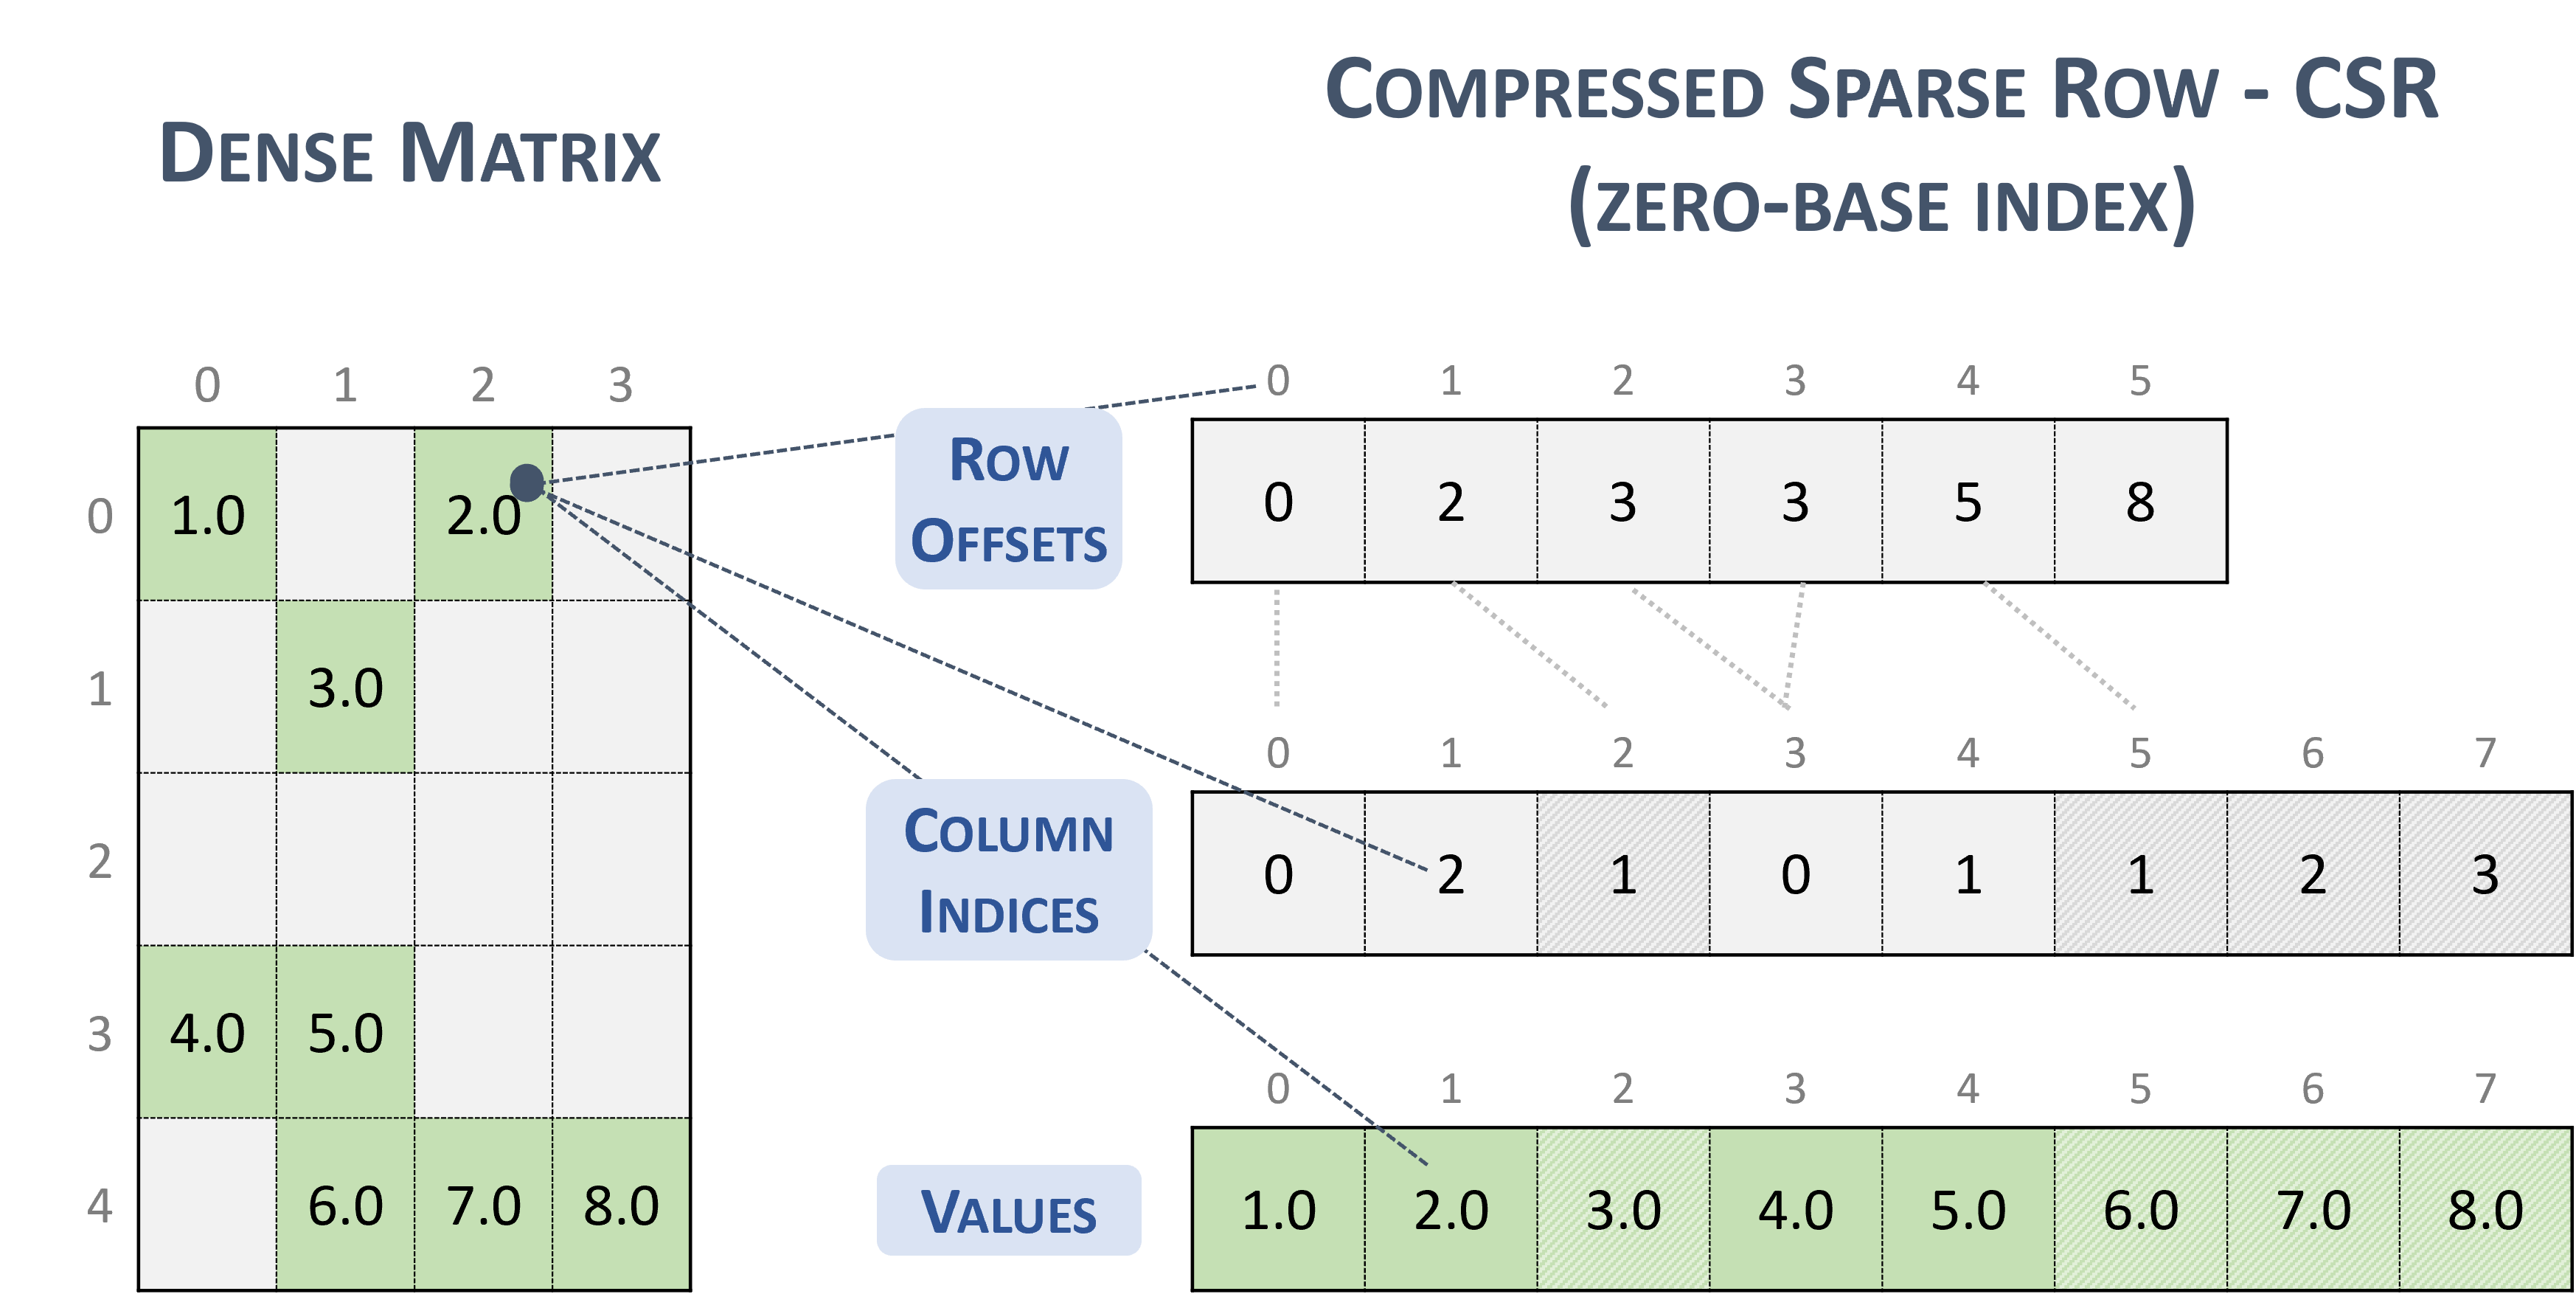
\includegraphics[width=0.5\textwidth]{csr-format.png}
        \label{fig:csr-format}
    \end{figure}

    This format consists of three arrays used to store the rows, columns and
    non-zero values of the matrix, the main advantage is that the array
    containing the row indices is constructed by sorting and creating a prefix
    sum of the original row indices reducing the length of the row array from
    the number of non-zero to the number of rows plus one.

    Using the CSR format, access to the $i$-th row can be obtained just by
    taking the $i$-th value of the row array as shown in figure
    \ref{fig:csr-format}.

    \section{Parallelization}

    Starting from a full CPU implementation as baseline, an optimized CPU and
    four different CUDA implementation were developed, each one being a
    variation of the previous one taking into account a specific group of
    operations.

    \subsection{OpenMP}

    Using the OpenMP library the naive CPU implementation can be improved by
    parallelizing the operation on multiple CPU threads.

    \subsection{One Thread Per Row}

    For the first CUDA implementation, since each value of the output array can
    be calculated independently from the others, the naive approach is to
    create a single thread for each row which multiplies all its non-zero
    values with the corresponding input vector elements and sums them together
    sequentially.

    \subsection{Additional Sorting Kernel}

    Since the CSR format requires sorting, for large matrices a lot of time is
    spent for the construction of the row array of the matrix so as a solution
    a \textbf{Bitonic Parallel Sort} algorithm was implemented to achieve
    faster execution time.

    \subsection{One Thread Per Non-Zero}

    For matrices having long rows the naive implementation can be slow so as an
    alternative approach the matrix can be subdivided into chunks having one
    thread for each non-zero value.

    The main difficulties of this approach are the subdivision of the matrix
    into groups to balance the workload and the additional \textbf{concurrency}
    problem caused by access to the same memory region between multiple threads.

    As a naive solution for the concurrency problem, mainly caused by the sum
    of the products, each product is stored inside the matrix itself and the
    sum is executed sequentially on the CPU.

    \subsection{Warp Reduction}

    A better solution to the previous problem is to exploit modern warp
    \textbf{reduction primitives} to parallelize the sum operations hence
    increasing performance of the algorithm.

    \section{State of the Art}

    From the original Compressed Sparse Row (CSR) \cite{eisenstat1977csr}
    implementation many more research has been conducted to improve its use in
    algorithms such as Sparse Matrix-Vector Multiplication.

    One of the main problems of the format was its performance which is
    \textbf{highly dependent} on the used hardware and the actual structure of
    the matrix.
    To achieve this, several optimized variants of CSR have been developed such
    as CSR5 and its extension CSR5BC which improve parallelism and memory
    access on modern GPUs using segmented sum techniques and index compression
    \cite{zhang2016csr5}.

    The CSR\&RV format reduces memory usage by storing redundant values only
    once, significantly lowering storage costs and boosting throughput
    \cite{tang2023csrrv}.

    On heterogeneous systems, formats like CSR-k restructure data
    hierarchically for better adaptability across CPUs and GPUs
    \cite{liu2022csrk}.
    Auto-tuning frameworks such as AlphaSparse generate customized kernels
    tailored to both sparsity patterns and hardware, delivering further gains
    \cite{yin2022alphasparse}.

    Additionally, emerging architectures like Processing-In-Memory (PIM) are
    prompting new SpMV implementations, such as SparseP, that harness in-memory
    computing advantages \cite{lee2022sparsep}.
    Together, these innovations demonstrate that while CSR remains foundational,
    ongoing adaptations are essential for maximizing SpMV efficiency on
    evolving platforms.

    \section{Methodology and Contributions}\label{sec:methodology}

    For profiling on the CPU the \texttt{gettimeofday} function was used to
    measure the time taken by different operations down to the microseconds,
    such as memory allocation, matrix file parsing, input vector value generation,
    etc....

    For the GPU \textbf{CUDA events} were used instead to achieve
    \textbf{better accuracy} for the elapsed time including the internal
    synchronization of the threads.

    \begin{algorithm}[h!]
        \caption{Naive GPU SpMV kernel}
        \algorithmicrequire~The input matrix $A$ of size $n \cdot m$ and the vector $x$ of size $m$.
        \begin{algorithmic}[1]
            \Procedure{SPMV}{$A$, $x$, $n$, $m$}
                \State $y \gets \emptyset$
                \For{$r$ in $\{1 \dots n\}$ \textbf{parallel}}
                    \For{$c$ in $\{1 \dots m\}$}
                        \State $y[r] += A[r * m + c] + b[c]$
                    \EndFor
                \EndFor
                \State \textbf{return} $y$\Comment{the result vector}
            \EndProcedure
        \end{algorithmic}
        \label{alg:SpMVrow}
    \end{algorithm}
    The naive GPU kernel implementation is expected to be \textbf{slower} for
    long row matrices since the SpMV becomes almost sequential, which can be
    seen in the algorithm \ref{alg:SpMVrow}

    \begin{algorithm}[!ht]
        \caption{Warp reduction SpMV kernel}
        \algorithmicrequire~The input matrix $A$ of size $n \cdot m$ and the vector $x$ of size $m$.
        \begin{algorithmic}[1]
            \Procedure{SPMV}{$A$, $x$, $n$, $m$}
                \State $y \gets \emptyset$
                \For{$i$ in $\{1 \dots n \cdot m\}$ \textbf{parallel}}\Comment{product only}
                    \State $c \gets cols[i]$
                    \State $A[i] *= x[c]$
                \EndFor

                \For{$warp$ in $\{1 \dots n \cdot m / 32 \}$ \textbf{parallel}}\Comment{warp reduction}
                    \State $val \gets A[warp \cdot 32]$
                    \For{$off$ in $\{16, 8, 4, 2, 1\}$} 
                        \For{$j$ in $\{1 \dots 32 \}$ \textbf{parallel}}
                            \State $val += A[warp * 32 + j]$
                        \EndFor
                    \EndFor
                    \State $A[warp \cdot 32] = val$
                \EndFor

                \For{$r$ in $\{1 \dots n\}$}\Comment{sum of the reductions}
                    \For{$c$ in $\{1 \dots m / 32\}$}
                        \State $y[r] += A[r \cdot m + c \cdot 32]$
                    \EndFor
                \EndFor

                \State \textbf{return} $y$\Comment{the result vector}
            \EndProcedure
        \end{algorithmic}
        \label{alg:SpMVnz}
    \end{algorithm}

    The other approach using one thread for each non-zero element is expected
    to be more \textbf{consistent} across different matrices and slightly
    faster than its naive counterpart since it is also able to parallelize the
    sums even if the implemented algorithm can still be improved.

    \section{System Description and Experimental Set-up}
        \subsection{System Description}

        For the development of the project the following requirements were used
        inside the university cluster:
        \begin{itemize}
            \item SLURM 32.11.3
            \item CUDA 12.1
            \item GCC 12.3.0
            \item GNU Make 4.3
            \item OpenMP 17.0.6
            \item Eigen 12.3.0 (for the utilities)
            \item Python 3.9.18 (for the utilities) 
        \end{itemize}

        The project can be compiled using the provided Makefiles with GCC and
        CUDA compilers and can be run into the cluster via the SLURM workload
        manager utilities.

        \begin{table}[ht]
            \caption{System details}
            \label{tab:system_description}
            \centering
            \begin{adjustbox}{width=\columnwidth}
            \begin{tabular}{lllrl}
            \toprule
            \textbf{System} &  \textbf{Processor} & \textbf{Cores per Socket} & \textbf{RAM} & \textbf{Accelerator} \\
            \midrule
                laptop & Intel(R) Core(TM) i5-1035G1 CPU & 4 at 3.6 GHz & 8 GB & Intel Iris Plus Graphics G1 (Ice Lake) \\
                baldo & Intel(R) Xeon(R) Silver 4214 CPU & 12 at 2.2 GHz & 405 GB & \\
                edu-short & AMD EPYC 9334 32-Core Processor & 32 at 3.9 GHz & 810 GB & NVIDIA L40S \\
            \bottomrule
            \end{tabular}
            \end{adjustbox}
        \end{table}

        \subsection{Dataset description}
        
        Eight different matrices were selected as dataset, each with specific
        characteristics to evaluate the performance of the various
        implementations.

        The first five matrices are mostly symmetric and differ primarily in
        the number of non-zero elements, which increases progressively from one
        matrix to the next.

        The \texttt{heart1} matrix stands out for its \textbf{higher density},
        with non-zero values accounting to approximately 10\% of the total
        entries.

        The final two matrices are asymmetric and are designed to stress test
        different dimensions: one has a large number of rows, while the other
        has a large number of columns.

        \begin{table}[ht]
            \caption{Matrix Details}
            \label{tab:matrix_details}
            \centering
            \begin{adjustbox}{width=\columnwidth}
            \begin{tabular}{lrrrr}
            \toprule
            \textbf{Name} & \textbf{Rows} & \textbf{Columns} & \textbf{Non-Zeros} & \textbf{Symmetric} \\
            \midrule
                \textbf{1138\_bus} & 1,138 & 1,138 & 4,054 & Yes \\
                \textbf{bcsstk15} & 3,948 & 3,948 & 117,816 & Yes \\
                \textbf{bcsstk31} & 35,588 & 35,588 & 1,181,416 & Yes \\
                \textbf{pwtk} & 217,918 & 217,918 & 11,524,431 & Yes \\
                \textbf{cage15} & 5,154,859 & 5,154,859 & 99,199,551 & No \\
                \textbf{heart1} & 3,557 & 3,557 & 1,385,317 & No \\
                \textbf{relat8} & 345,688 & 12,347 & 1,334,038 & No \\
                \textbf{connectus} & 512 & 394,792 & 1,127,525 & No \\
            \bottomrule
            \end{tabular}
            \end{adjustbox}
        \end{table}

        \subsection{Experimental Set-up}

        For the experimental setup, each main operation is profiled by
        measuring its \textbf{execution time}.
        
        The profiled operations include:
        \begin{enumerate}
            \item Memory allocation and copy
            \item File Input/Ouput
            \item Sorting for CSR matrix construction
            \item Matrix-Vector multiplication
        \end{enumerate}

        The CSR matrix is constructed only once at the start of the program.
        To enure accurate timing of the matrix-vector multiplication, four
        initial \textbf{warm-up cycles} are executed and excluded from
        profiling.
        At the end the average value between 10 different runs is evalueted.

    \section{Experimental Results}

    The results for the different implementations across all matrices are shown
    in the following graphs.

    A few important points should be noted:
    \begin{itemize}
        \item Results for the CPU and naive GPU implementations on larger
            matrices are missing.
            This is because their total execution time exceeded the 5-minute
            time limit enforced by the cluster;
        \item The Y-axis of the graph uses a \textbf{logarithmic scale} rather
            than a linear one.
    \end{itemize}

    The logarithmic scale is necessary because the first five matrices increase
    in size by roughly an order of magnitude each, leading to similarly scaled
    increases in execution times.

    \begin{figure}[ht]
        \caption{Full Time Benchmark}
        \centering
        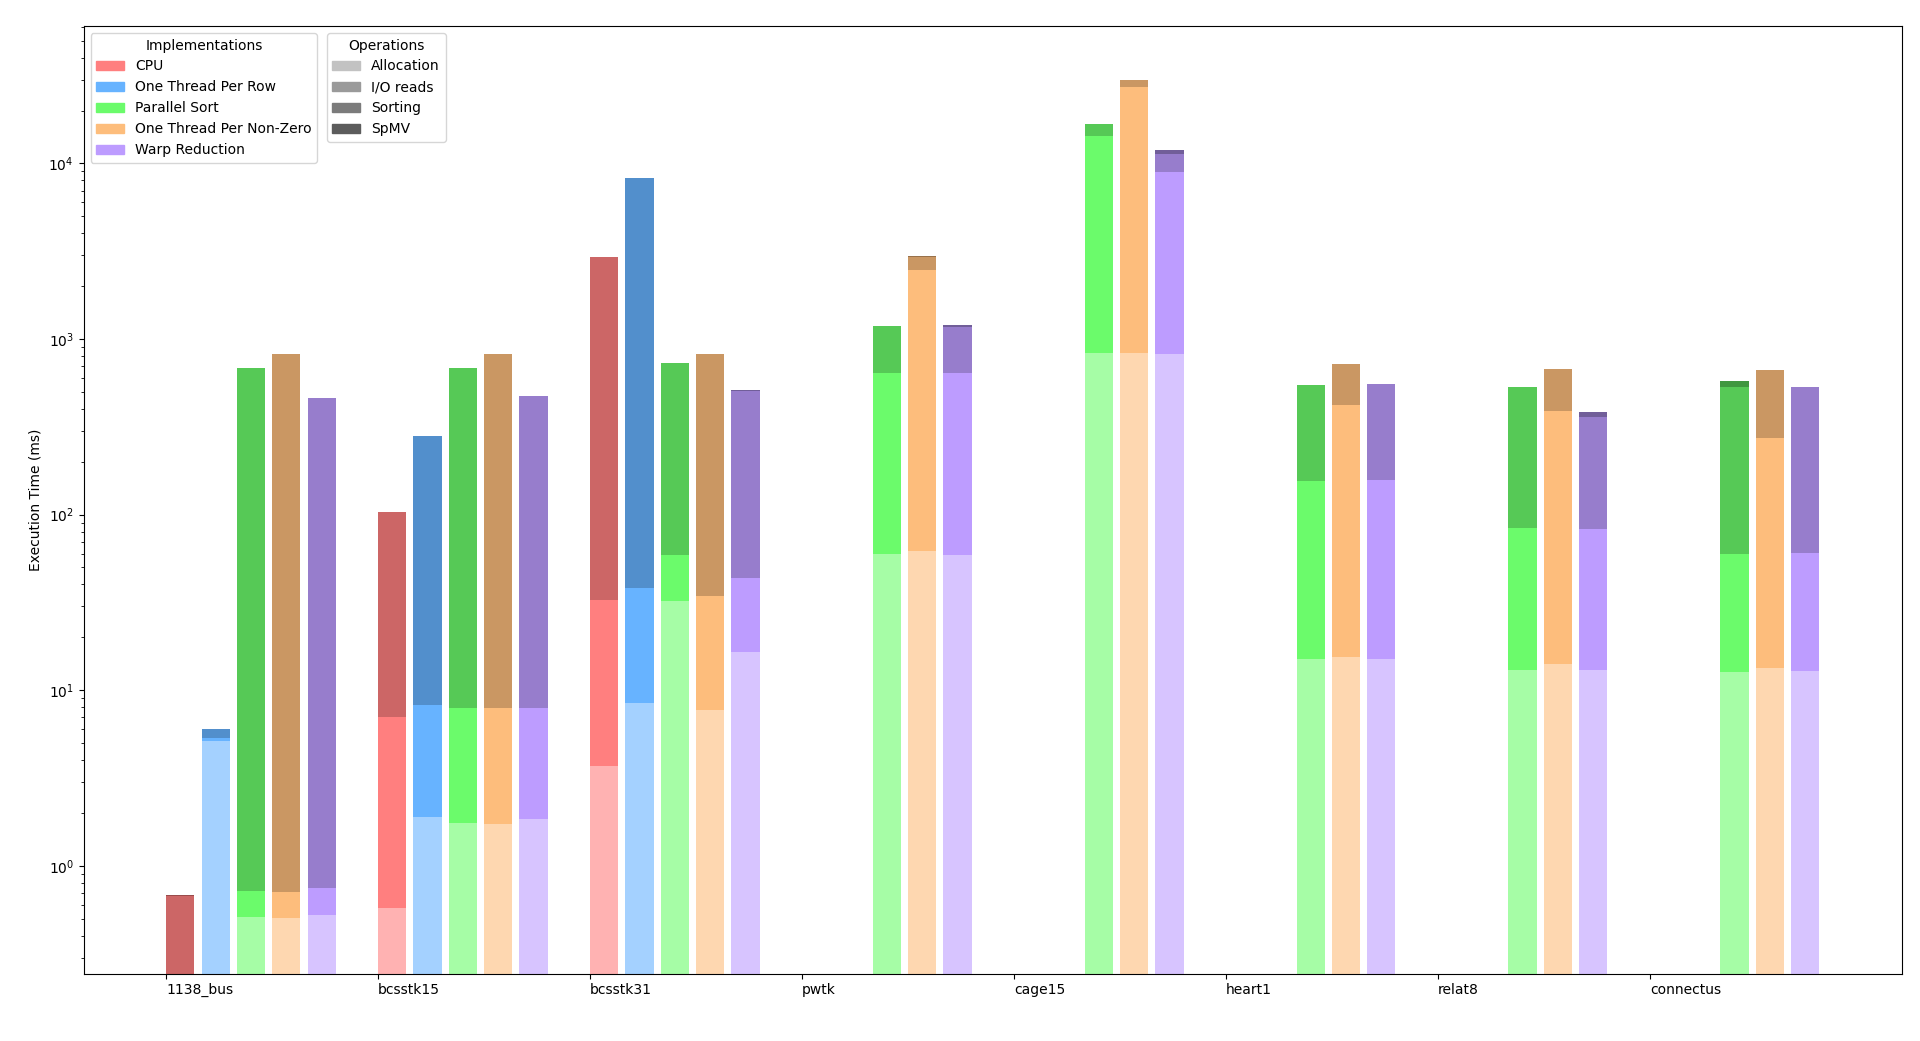
\includegraphics[width=0.5\textwidth]{full-benchmark.png}
        \label{fig:full-benchmark}
    \end{figure}

    From the results, we can observe that the CPU implementation performs
    better on smaller matrices, primarily due to the \textbf{lower overhead}
    compared to the GPU (e.g. memory allocation and kernel dispatch).
    However, its performance degrades rapidly as the number of non-zero
    elements increases.

    As shown in figure \ref{fig:spmv-benchmark} using OpenMP increases by a
    little margin the performance of the algorithm even if not as much as
    expected.

    Since sorting the matrix rows for CSR construction takes a significant
    portion of the total time, using a Bitonic Parallel Sort considerably
    reduces overall execution time.

    Other \textbf{performance-impacting factors} include memory allocation and
    data transfer, especially between host and device, as well as file I/O
    operations.
    These are areas that could benefit from further optimization.

    \begin{figure}[ht]
        \caption{SpMV Time Benchmark}
        \centering
        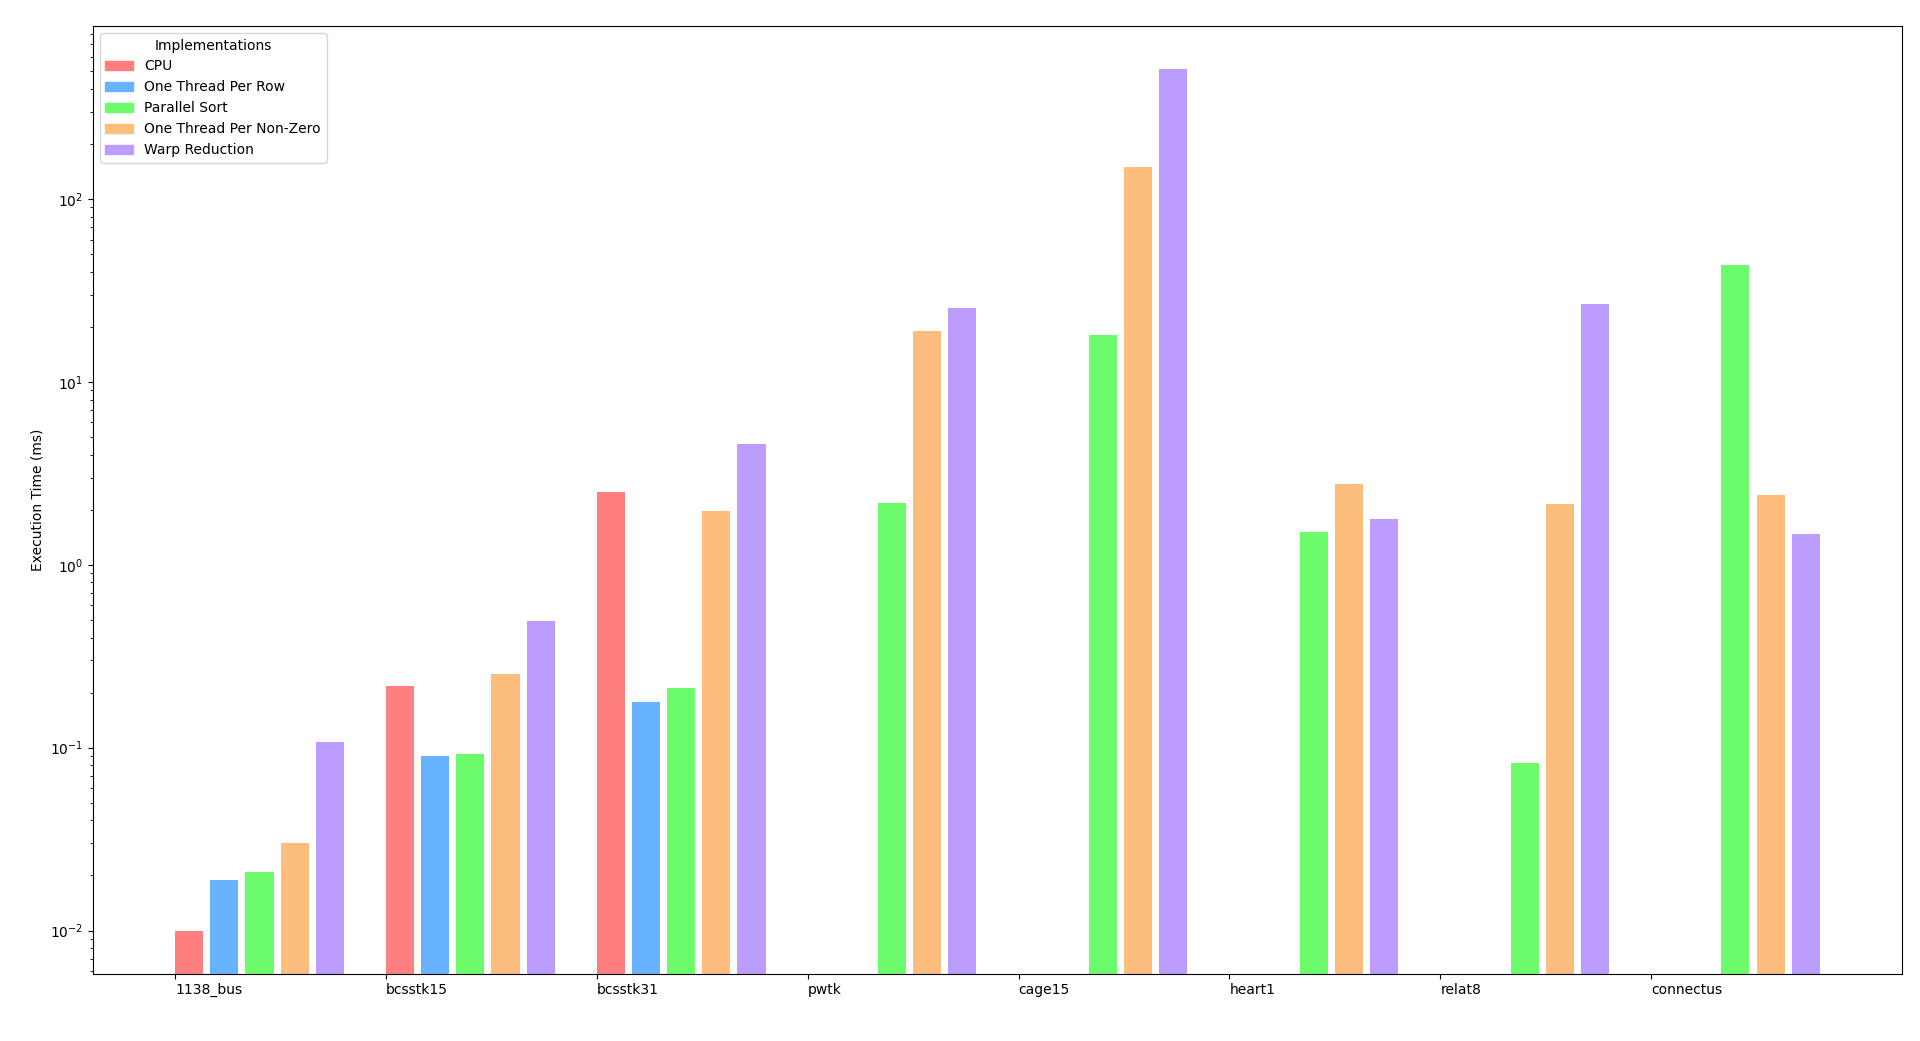
\includegraphics[width=0.5\textwidth]{spmv-benchmark.png}
        \label{fig:spmv-benchmark}
    \end{figure}

    As expected, using one thread per row yields better performance on matrices
    with a large number of rows (e.g. \texttt{relat8}).
    However, it performs poorly on matrices with fewer but longer rows (e.g.
    \texttt{connectus}).

    On the other hand, using one thread per non-zero element delivers more
    consistent performance across different matrix shapes.
    Nevertheless, since this approach requires the summation of partial
    products to be performed on the CPU (to avoid race conditions due to
    concurrent memory access), it is often slower than the one-thread-per-row
    implementation.

    The warp reduction strategy, which partially parallelizes the summation
    process, shows \textbf{limited performance improvement}.
    This is expected, as only one full reduction is performed on the device for
    each warp, while the remaining summation still occurs on the host.
    This bottleneck is especially evident in the case of the \texttt{relat8}
    matrix, where the high number of rows leads to more CPU-side operations.

    \section{Conclusion}

    To summarize, parallelizing both the sorting phase and the matrix-vector
    product on the GPU significantly improves performance for large sparse
    matrix-vector multiplications (SpMV).

    While the one-thread-per-row approach generally delivers better performance,
    the one-thread-per-non-zero implementation has potential for 
    textbf{further optimization} and could be improved to achieve lower
    execution times.

    Looking ahead, future work could explore \textbf{adaptive} or hybrid
    algorithms that dynamically select the most suitable strategy based on the
    specific characteristics of each matrix, as well as different approaches to
    balance the parallel operations across all the elements of the matrix.

    \bibliographystyle{IEEEtran}
    \bibliography{references}

\end{document}
